% !TeX spellcheck = de_DE
\documentclass{alex_gp}

\name{Alexander Helbok}
\course{Grundpraktikum}
\hwnumber{3}
\spacing{}
\usepackage{makecell}

\begin{document}
\renewcommand{\labelenumi}{\alph{enumi})}


\begin{mybox}{Eine Feder mit drei Massen}
	Bei diesem Versuch, wurde mit Federn experimentiert, um den Zusammenhang zwischen Masse und Schwingungsdauer zu ermitteln. Dafür wurden verschiedene Massen an eine Feder gehängt und in Schwingung gebracht. Während der Schwingung haben Sensoren die Beschleunigung und die Kraft auf die Feder gemessen und aufgezeichnet. 
	
	Der Versuchsaufbau sah wie folgt aus: 
	An eine Sessellehne war ein Haken befestigt, auf welches ein Stück Karton gesteckt wurde. Der Karton dient hier als Steckbrett für Federn, damit mehrere Federn für spätere Versuche parallel geschalten werden können. In den Karton stecken wir zunächst eine einzelne Feder, an welches andere Ende, wieder über ein Stück Karton, das IOLab am Kraftsensor aufgehängt wurde. 
	
	Um die Masse des Pendelkörpers zu bestimmen, wurde das IOLab an einer Schnur aus der Ruhelage hochgezogen. Dabei wurde die Beschleunigung und die Kraft in vertikaler Richtung gemessen und nach Newtons zweitem Axiom gilt dann für die Masse
	\begin{equation}\label{eqn:newt}
		m = \tfrac{F}{a} 
	\end{equation}
	Für die gemessene Beschleunigung \( a \) wird ein Fehler von \( 0.001 \unit{\a} \) angenommen, da das die Genauigkeit ist, mit der die Beschleunigung im Programm angegeben wird. Der Kraft \( F \) wird ein Fehler von \( 0.0025 \unit{N} \) zugesprochen, weil der Sensor ein Auflösungsvermögen von \( 0.005 \unit{N} \) hat. In Abbildung \ref{fig:mass} ist die Bestimmung einer Masse (Dritten und Schwersten) dargestellt.
	\begin{figure}[H]
		\vspace{-1cm}		
		\centering
		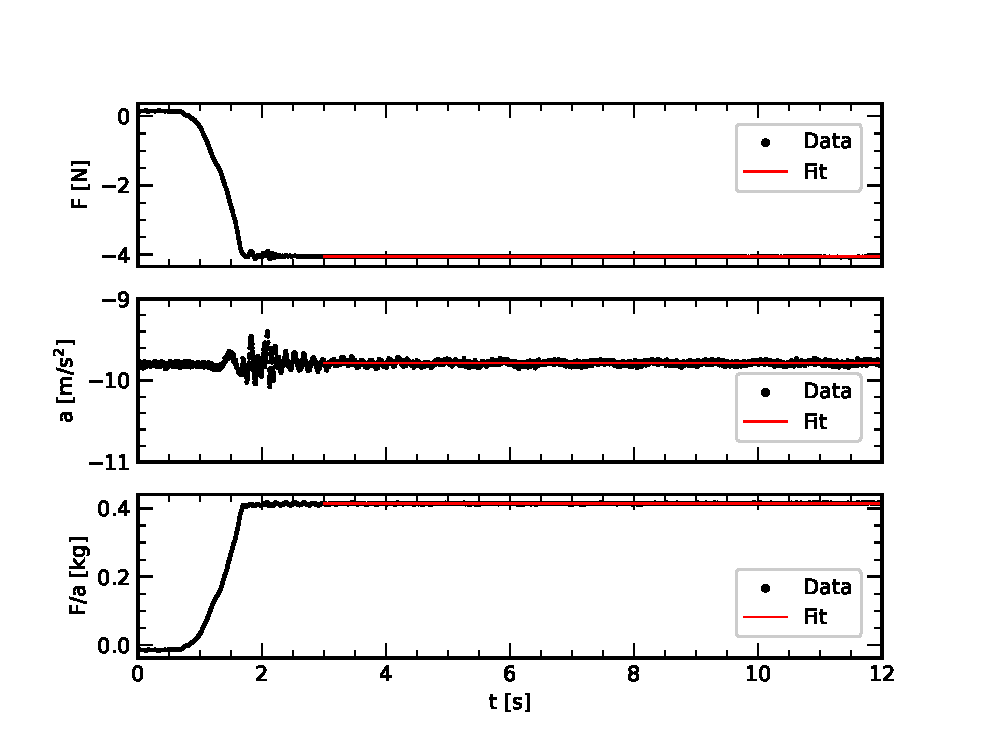
\includegraphics[width=0.9\textwidth]{Versuch3_1.eps}
		\caption{Vom oben nach unten sind Kraft \( F \), Beschleunigung \( a \) und die Masse als Quotient zwischen Kraft und Beschleunigung \( F/a \) aufgetragen. Die Fehlerbalken der Daten sind zu klein, um sie auszumachen und werden daher nicht eingetragen. Die drei Grafiken teilen sich die horizontale Achse. Zudem sind in Rot Geraden von \( t = 3 \unit{s} \) bis \( t = 12 \unit{s} \) angepasst.}
		\label{fig:mass}
	\end{figure}
	
	Hängt man das IOLab an eine Feder und lenkt diese aus, fängt das System an zu Pendeln. Diese Schwingungen lassen sich mittels Beschleunigungs- und/oder Kraftsensors aufzeichnen und aus ihnen kann man charakteristische Eigenschaften der Oszillation, wie die Schwingungsdauer \( T \) oder die Kreisfrequenz \( \omega \), bestimmen. Dafür wurde eine Sinuskurve der Form \( f(x) = A\sin(\omega x + \phi) + d \) mit einem Fitprogramm an die Messpunkte angepasst, wobei die an SciPy übergebenen Daten nur „schöne“ Schwingungen enthalten.
	
	Für die Analyse der Schwingungsdaten wurde der Beschleunigungssensor verwendet, da dieser ein höheres Auflösungsvermögen als der Kraftsensor hat. In Abbildung \ref{fig:sine} sieht man die ersten und letzten sechs Sekunden der Messung und eine an die Beschleunigungsdaten angepasste Sinuskurve. Die Amplituden stimmen nicht ganz überein, da die Maxima und Minima aufgrund von Reibung und Luftwiderstand mit der Zeit abnehmen und dies im Sinusfit nicht berücksichtigt wird. Die Amplitude der angepassten Kurve kann man sich als den Mittelwert aller Maxima vorstellen und ist daher zu Beginn der Messung etwas zu Niedrig und gegen Ende zu Groß. Dies spiegelt sich aber nur in der Unsicherheit der Amplitude \( A \) des Fits wieder und nicht in der des Parameters \( \omega \).
	
	\begin{figure}[H]
		\centering
		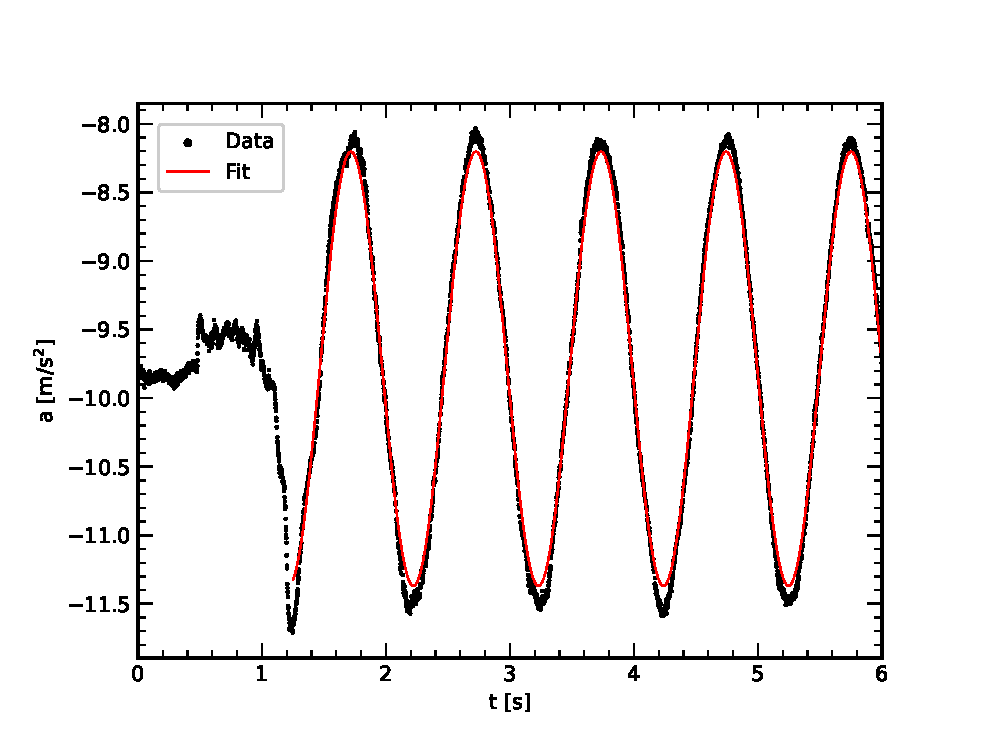
\includegraphics[width=1\textwidth]{Versuch3_2.eps}
		\caption{Die Beschleunigung wurde auf die Zeit aufgetragen und eine Sinuskurve in Rot wurde an die Daten ab \( t = 1 \unit{s} \) (bis \( t = 41.5 \unit{s} \)) angepasst. Die Fehlerbalken der Daten sind zu klein, um sie auszumachen und werden daher nicht eingetragen.}
		\label{fig:sine}
	\end{figure}
	
		Es wurden 3 Versuche mit unterschiedlichen Massen und gleicher Feder durchgeführt. Dafür wurde mit Klebeband zunächst ein und dann zwei Steine ans Messgerät geklebt und wieder an die gleiche Feder gehängt. In Tabelle \ref{table:1} sind Masse, Wurzel der Kehrwerts der Masse, Periode und Winkelfrequenz der verschiedenen Versuche mit dazugehörigen Fehlern aufgelistet. \par
	\begin{center}
		\captionof{table}{Gemessene Masse, Schwingungsdauer, Winkelfrequenz und Federkonstante der drei Versuche}
	%	\begin{tabular}{@{}r c r c r c r @{}}\toprule
	%		&& Versuch1 && Versuch 2 && Versuch 3 \\ \midrule
	%		\( m \) [kg] && 0.2030(11) && 0.3549(2) && 0.4146(2) \\
	%		\( \sqrt{1/m}\; [\text{kg}^{-\tfrac{1}{2}}] \) && 2.220() && 1.677() && 1.553() \\
	%		T [s] && 0.75465(4) && 0.93366(7) && 1.0083(1) \\
	%		$\omega$ [s\( ^{-\tfrac{1}{2}} \)] && 8.8759(4) && 6.7297(5) && 6.2316(6) \\
	%		\bottomrule
	%	\end{tabular}
		\begin{tabular}{@{\extracolsep{5mm}} 
				r
				S[table-format=1.5(1)]
				S[table-format=1.5(1)]
				S[table-format=1.5(1)]
			}
			\toprule
			\makecell[t]{}
			&   {\makecell[t]{Versuch 1}}
			&   {\makecell[t]{Versuch 2}}
			&   {\makecell[t]{Versuch 3}}\\
			\midrule
			\( m \) (kg) & 0.2030(11) & 0.355(2) & 0.415(2) \\
			\( \sqrt{1/m}\; (\sqrt{1/\unit{kg}}) \) & 2.219(6) & 1.679(5) & 1.553(4) \\
			T (s) & 0.70789(4) & 0.93366(7) & 1.00829(10) \\
			$\omega$ (1/s) & 8.8759(4) & 6.7297(5) & 6.2316(6) \\
			\( k \) (N/m) & 15.99(9) & 16.074(99) & 16.10(8) \\
			\bottomrule
		\end{tabular}
	\label{table:1}
	\end{center}

	Das Federpendel wird näherungsweise durch einen harmonischen Oszillator beschrieben. In diesem Modell wird eine Konstante \( k \) eingeführt, welche die Winkelfrequenz \( \omega \) und die Masse \( m \) in Verbindung setzt. Aus dem Modell gehen folgende Zusammenhänge hervor:
	\begin{equation}\label{eqn:k}
		k = \omega^2 m \quad \Leftrightarrow\quad \omega = \sqrt{k}\sqrt{1/m}
	\end{equation}
	\( \sqrt{k} \) ist also die Proportionalitätskonstante zwischen \( \omega \) und \( m \). Dies wird in Abbildung \ref{fig:sqrt} anhand der in Tabelle \ref{table:1} angegebenen Werten illustriert. Zusätzlich zu den drei Datenpunkten wurde eine Gerade, wie sie das Modell vorhersagt, angepasst, wodurch man für die Steigung der linearen Funktion \( \sqrt{k} = 4.005(4) \unit{\sqrt{kg / s^2}} \) erhält.
	\begin{figure}[H]
		\centering
		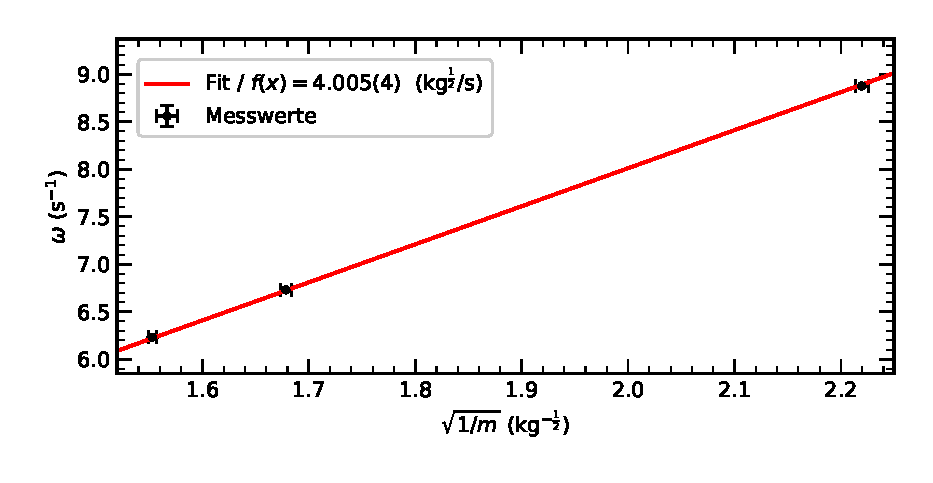
\includegraphics[width=\textwidth]{Versuch3_3.eps}
		\caption{Winkelfrequenz für drei unterschiedliche Massen. In rot wurde eine lineare Funktion durch den Ursprung angepasst. Die Fehlerbalken stellen den 1$\sigma$ Fehler dar; die Unsicherheit in \( \omega \) ist so gering, dass sie kaum sichtbar ist.}
		\label{fig:sqrt}
	\end{figure}
	Aus der angepassten Gerade erhält man durch quadrieren \( k = 16.04(3) \unit{N/m} \). Dieser Wert lässt sich gut mit den mittels Gleichung \ref{eqn:k} berechneten Werte für die drei Massen (Siehe Tabelle \ref{table:1}) vereinbaren und bestätigt das Modell des harmonischen Oszillators bzw. den linearen Zusammenhang zwischen dem Quadrat der Winkelfrequenz $\omega$ und dem Kehrwert der Masse \( m \). 

	Eine Federkonstante von \( k_1 = 8(1) \unit{N/m} \), welche ein anderer Kursteilnehmer gemessen hat, ist nicht mit den hier präsentierten Ergebnissen vereinbar. Di beiden Werte liegen mehrere Standardabweichungen voneinander entfernt und können daher nicht durch statistische Schwankungen erklärt werden. Eine mögliche Erklärung für diese Situation ist, dass die Annahme, das alle Federn im Labor gleich sind, falsch ist, da zum Beispiel durch Überdehnung einer Feder dessen Federkonstante permanent reduziert wird. Der andere Kursteilnehmer könnte eine solche Feder für seinen Versuch verwendet haben.
\end{mybox}

\begin{mybox}{Entwicklung eines Modells für parallele Federn}
	Die Folgenden Experimente versuchen die Frage zu beantworten, wie sich das Pendel verhält, wenn man mehrere Federn kombiniert und wie sich das auf die Federkonstante des Oszillators auswirkt. Dafür wurde zunächst eine zweite Feder ins Steckbrett aus Karton gesteckt, sodass jetzt das Messgerät über zwei Federn an der Sessellehne aufgehängt ist. Die Masse wurde bei der Schwersten aus dem vorherigen Versuch festgehalten (\( m = 0.4146(2) \unit{kg} \)).
	
	Die Kreisfrequenz wurde analog wie im vorherigen Versuch über eine Sinuskurve ermittelt. Die gemessenen Werte für \( \omega, T \) und \( k \) sind in Tabelle \ref{table:2} eingetragen.
	
	\begin{center}
		\captionof{table}{Gemessene Schwingungsdauer, Winkelfrequenz und Federkonstante bei verschiedener Anzahl an Federn}
		\begin{tabular}{@{\extracolsep{5mm}} 
				r
				S[table-format=2.5(1)]
				S[table-format=2.5(1)]
				S[table-format=2.5(1)]
			}
			\toprule
			\makecell[t]{}
			&   {\makecell[t]{1 Feder}}
			&   {\makecell[t]{2 Federn}}
			&   {\makecell[t]{3 Federn}}\\
			\midrule
			T (s) & 1.00829(10) & 0.71903(4) & 0.59264(3) \\
			$\omega$ (1/s) & 6.2316(6) & 8.7384(5) & 10.6021(5) \\
			\( k \) (N/m) & 16.10(8) & 31.7(2) & 46.6(2) \\
			\bottomrule
		\end{tabular}
		\label{table:2}
	\end{center}
	
	Der ermittelte Wert für die Federkonstante für zwei Parallele Federn ist im Rahmen der Unsicherheit doppelt so groß wie der einer einzelnen Feder. Man könnte daher die Vermutung aufstellen, dass die kombinierte Federkonstante linear mit der Anzahl der Federn skaliert und man folgenden Zusammenhang erhält:
	\begin{equation}\label{eqn:paral}
		k_{\text{ges}} = Nk
	\end{equation}
	wobei \( N \) die Anzahl der verwendeten Federn ist. 
	
	Um diese Hypothese zu testen, wurde eine weitere Feder dazugehängt und das bereits beschriebene Prozedere durchlaufen, um die Frequenz der Schwingung zu ermitteln. 
	
	\begin{figure}[H]
		\centering
		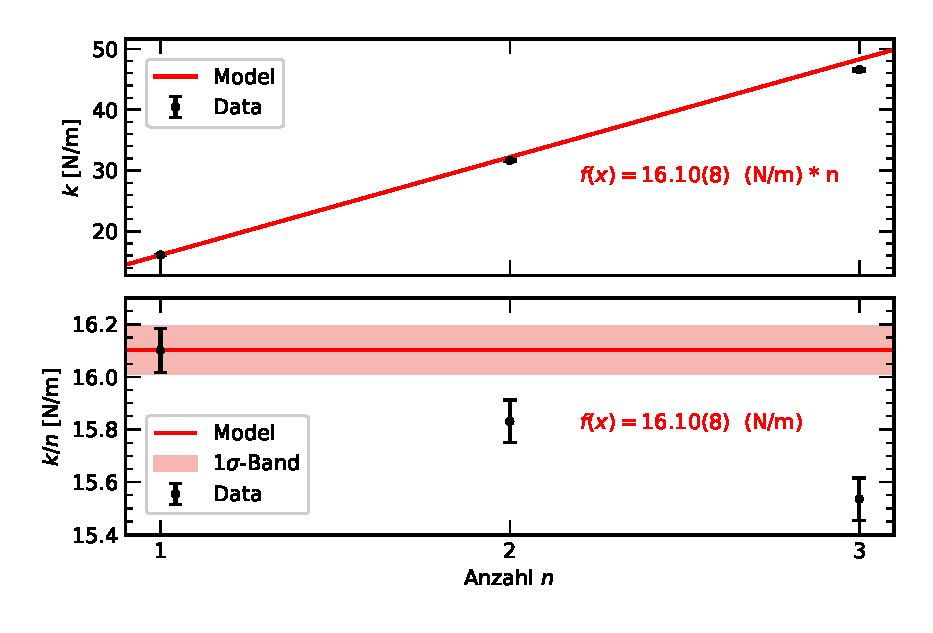
\includegraphics[width=\textwidth]{Versuch3_4.eps}
		\caption{Winkelfrequenz für drei unterschiedliche Massen. In rot wurde eine lineare Funktion durch den Ursprung angepasst. Die Fehlerbalken stellen den 1$\sigma$ Fehler dar; die Unsicherheit in \( \omega \) ist so gering, dass sie kaum sichtbar ist.}
		\label{fig:k2}
	\end{figure}
	
	
%	\begin{tabular}{@{}r | r @{}}\toprule
%		N & \( \omega [\text{s}^{-1}]\) \\ \midrule
%		1 & 16.115() \\
%		2 & 31.664() \\
%		3 & 46.614() \\
%		\bottomrule
%	\end{tabular}
\end{mybox}

\end{document}